\documentclass[12pt]{article}
\usepackage{amssymb,amsfonts,amsmath,amsthm}
\usepackage[utf8]{inputenc}
\usepackage[T1]{fontenc}
\usepackage{graphicx}
\usepackage{listings}
\usepackage{float}
\usepackage[ruled]{algorithm2e}
\usepackage[noend]{algpseudocode}
\usepackage{numberedblock}
\usepackage{lipsum}
\usepackage[autostyle]{csquotes}
\usepackage{hyperref}

\lstdefinelanguage{JavaScript}{
  keywords={typeof, new, true, false, catch, function, return, null, catch, switch, var, if, in, while, do, else, case, break},
  keywordstyle=\color{blue}\bfseries,
  ndkeywords={class, export, boolean, throw, implements, import, this},
  ndkeywordstyle=\color{darkgray}\bfseries,
  identifierstyle=\color{black},
  sensitive=false,
  comment=[l]{//},
  morecomment=[s]{/*}{*/},
  commentstyle=\color[rgb]{0, 0.4, 0}\ttfamily,
  stringstyle=\color[rgb]{0.4, 0, 0}\ttfamily,
  morestring=[b]',
  morestring=[b]"
}
\lstset{
   language=JavaScript,
   backgroundcolor=\color{white},
   extendedchars=true,
   basicstyle=\footnotesize\ttfamily,
   showstringspaces=false,
   showspaces=false,
   numbers=left,
   numberstyle=\footnotesize,
   numbersep=9pt,
   tabsize=2,
   breaklines=true,
   showtabs=false,
   captionpos=b
}

\newlength\mylen
\newcommand\myinput[1]{%
  \settowidth\mylen{\KwIn{}}%
  \setlength\hangindent{\mylen}%
  \hspace*{\mylen}#1\\}

\newcommand{\appname}{RuleVisualization}
\newcommand{\appnameit}{\textit{RuleVisualization}}
\newcommand{\appversion}{1.1.1}

\newcommand\norm[1]{\left\lVert#1\right\rVert}

\title{\appname \ \appversion \ -- User guide}
\author{Mateusz Lewandowski}

\begin{document}

\maketitle
\tableofcontents

\pagebreak

\section{Introduction}

\subsection{Installation}

Each released version of \texttt{RuleVisualization} application can be downloaded from \href{https://github.com/ruleLearn/RuleVisualization-release/releases}{https:github.com/ruleLearn/RuleVisualization-release/releases}, as a ZIP archive. After downloading the archive, one just needs to extract it to a directory of choice. No installation is required. Nevertheless, for the application to work one needs to have Java Runtime Environment (JRE) 8 or higher installed in the operating system.

\subsection{Running application}\label{subsec:server}

RuleVisualization consists of client and server applications. 
Requirements:
\begin{itemize}
    \setlength\itemsep{0em}
    \item Java 8 or higher (\texttt{java -version}),
    \item Internet browser. 
\end{itemize}

To run the application:
\begin{enumerate}
    \setlength\itemsep{0em}
    \item Run server on specified port number (8081 by default):\\
          \texttt{java -jar ./server/server.jar <port\_number> }
    \item Run client by opening \texttt{index.html} file in browser.
    \item Enter address of server URL on \texttt{index.html} webpage.
\end{enumerate}

%\subsection{Application development}
%
%Server development (Java, requires Java JDK 8 or higher):
%\begin{enumerate}
%    \setlength\itemsep{0em}
%    \item Compile project.\\
%          \texttt{mvn compile}
%    \item Modify code.
%    \item Generate JAR file into \texttt{target/server.jar}.\\
%          \texttt{mvn clean install}
%\end{enumerate}
%
%Client development (Vue.js; requires node.js):
%\begin{enumerate}
%    \setlength\itemsep{0em}
%    \item Install modules defined in \texttt{package.json} (first project run):\\
%          \texttt{npm install}
%    \item Enable hot reloading on \texttt{http://localhost:8080}: \\
%          \texttt{npm run serve}
%    \item Modify code.
%    \item Build application into \texttt{dist} folder:\\
%          \texttt{npm run build}
%\end{enumerate}

\pagebreak

\section{Setup}

\texttt{Setup} tab is used to load data as well as configure attributes and rule's characteristics. In general, four types of objects can be distinguished: attributes, rules, examples (objects), and characteristics (loaded along with rules). 

\subsection{Loading data}
Data can be loaded using the \texttt{Setup} tab -- see Fig. \ref{fig:setup}.
Data can be loaded from the local file system:
\begin{enumerate}
    \setlength\itemsep{0em}
    \item Enter URL for server application (see running server: \ref{subsec:server}).
    \item Browse for file with attributes (JSON format) -- required.
    \item Browse for file with rules (XML format) -- required.
    \item Browse for file with examples (JSON format) -- optional.
    \item Click \texttt{Load} button.
    \item After loading data: status message, main tabs, and configuration tabs will be displayed (or updated).
\end{enumerate}

\begin{figure}[H]
    \centering
    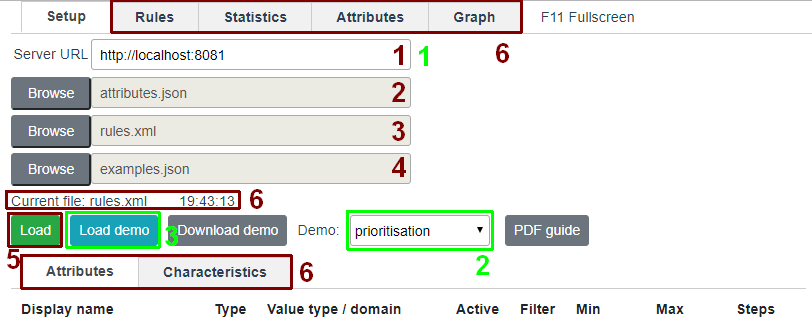
\includegraphics[width=\textwidth]{figures/setup.png}
    \caption{\texttt{Setup} tab}\label{fig:setup}
\end{figure}

Alternatively, data can be loaded from server demo data sets:
\begin{enumerate}
    \setlength\itemsep{0em}
    \item Enter \texttt{Server URL} (see running server: \ref{subsec:server}).
    \item Select a data set.
    \item Click \texttt{Load demo}.
    \item After loading data: status message, main tabs, and configuration tabs will be displayed (or updated).
\end{enumerate}

Format of files is compatible with format of files generated by \href{https://github.com/ruleLearn/rulelearn}{ruleLearn library}. In order to get familiar with that format, there is an option to download sample (demo) files by clicking \texttt{Download demo}.

After clicking \texttt{PDF guide}, it is possible to download most up-to-date version of this user documentation.

\subsection{Configuration (optional)}

Configuration enables user to configure loaded attributes and characteristics -- see Fig. \ref{fig:configure-attributes} and Fig. \ref{fig:configure-characteristics}. This step is fully optional and can be omitted. Names of particular attributes and characteristics can be adjusted to be displayed differently (e.g., in short or abbreviated) in \texttt{Filter} and \texttt{Match} tabs. \texttt{Type}, \texttt{Value type/domain}, \texttt{Active}, are properties of attributes loaded from JSON file, and are read only. Property \texttt{Filter} is used to show/hide characteristic or attribute in \texttt{Filter} tab. Property \texttt{Rules} is used to show/hide column with values of given characteristic in \texttt{Rules} tab. \texttt{Min} and \texttt{Max} are the minimum and maximum values in the domains of attributes or characteristics. They are used for: filtering (slider range) in \texttt{Filter} tab and for \textbf{computing similarity of rules and coloring edges/nodes} in \texttt{Graph} tab (based on domains' ranges). \texttt{Steps} are only used in \texttt{Filter} tab (number of steps determines how many intervals respective slider contains). Values \texttt{Min} and \texttt{Max} are initialized in the following way:
\begin{itemize}
    \setlength\itemsep{0em}
    \item for an attribute -- based on the loaded file with decision rules: minimal and maximal value in the set of all thresholds appearing in elementary conditions concerning this attribute,
    \item for a characteristic: using predefined values if the range for that characteristic is known a priori (e.g., \texttt{Strength} changes from 0 to 1), otherwise, based on the loaded file with decision rules (e.g., \texttt{Min} for \texttt{Support} is set to 0, and \texttt{Max} is set to maximum support value found among loaded rules).
\end{itemize}

\begin{figure}[H]
    \centering
    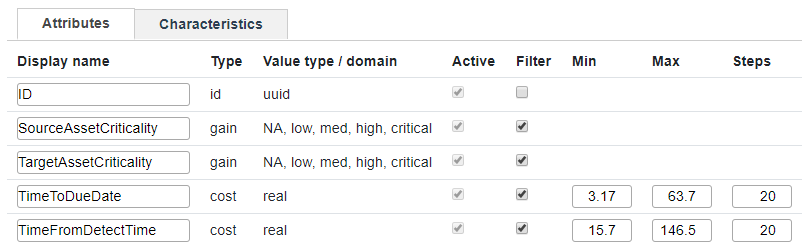
\includegraphics[width=\textwidth]{figures/configure-attributes.png}
    \caption{Configuration of attributes}\label{fig:configure-attributes}
\end{figure}

\begin{figure}[H]
    \centering
    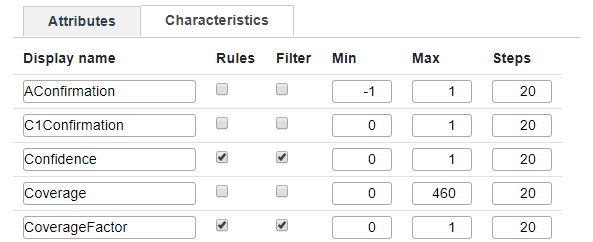
\includegraphics[width=\textwidth]{figures/configure-characteristics.png}
    \caption{Configuration of characteristics}\label{fig:configure-characteristics}
\end{figure}


\section{Filtering and matching rules}

Application stores in runtime: source ruleset (rules read from file), and context ruleset (source ruleset after applying filtering and matching). Filtering and matching can be used to change context rules. Context rules are always the same rules for all sections of application. It means that applying filter in one section (e.g. rules list), results in all other sections (graph, attributes matrix, statistics). Matching rules to objects can be interpreted as applying a filter.

\begin{figure}[H]
    \centering
    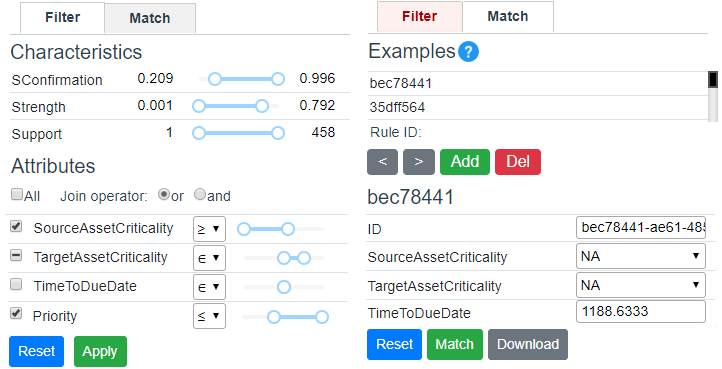
\includegraphics[width=\textwidth]{figures/B-filtering.png}
\end{figure}

Interpretation for filters selected on above figure:
\begin{quote}Select rules with SConfirmation between 0.209 and 0.996, Strength between 0.001 and 0.792, Support between 1 and 458. Every rule has to have condition C1 (with attribute SourceAssetCriticality, operator $\ge$, value between ``very low'' and ``high'') \textbf{or} decision C2 (with attribute Priority, operator $\le$ and value between 2 and 5). This rule mustn't contain condition C3 (with attribute TargetAssetCriticality and value between ``medium'' and ``high''.). Finally it has to also cover object ``bec78441''.
\end{quote}

Applying filters consists of:
\begin{itemize}
    \setlength\itemsep{0em}
    \item setting lower and upper limits of every characteristic that can occur in rule (applies after clicking Apply),
    \item setting occurrence (INCLUDE - tick, EXCLUDE - minus, IGNORE - blank), operator ($\le, \ge, \in$) and lower/upper limits of every attribute (applies after clicking Apply),
    \item selecting object, (covering filter applies after clicking Match button).
\end{itemize}

Mechanism of filtering insert rules from source ruleset into context ruleset. Every context rule:
\begin{enumerate}
    \setlength\itemsep{0em}
    \item ``contains'' at least one ``ticked'' attribute if JoinOperator = or, or, ``contains'' all ``ticked'' attributes if JoinOperator = and,
    \item not ``contains'' attributes with minus sign,
    \item may contain or may not contain blank attributes (without tick and minus) - these attributes are ignored and don't reduce context ruleset (operator and limits for this attributes are also ignored).
\end{enumerate}
``Contains'' means that, in rule, exists condition or decision with: chosen attribute, chosen operator and with value that is between limits. For instance when operator is equal $\ge$ and limits is $[2,5]$, it will match conditions/decisions: $\ge 2, \ge 3, \ge 4, \ge 5$. 

Operator $\in$ means: ANY operator. ``Reset'' button removes filter/match. If filtering or matching reduce source ruleset, then tab is red-colored (as on image).

\subsection{Match warning}\label{match}
Matching examples (selecting covering rules) is performed with use of Rule.covers method from rulelearn library. Examples can be edited by user. After modification, example is marked as ``dirty''. Clicking Match button sends all ``dirty'' objects to server in order to match rules again with ruleLearn library. \textbf{In order to refresh coverage similarity computations in rules graph, user is required for clicking ``Recompute'' in Graph tab}.

\section{Rules list}

This section represents list of context rules. After resetting filters and object matching, list displays all loaded decision rules. List has 3 features:
\begin{enumerate}
    \setlength\itemsep{0em}
    \item Sorting rules by characteristic value or length of condition part (by clicking on characteristic/conditions header of column),
    \item Enable/disable wrap of condition part content,
    \item Filtering covered examples by rule by clicking on rule's condition part (covered examples are displayed in Match section).
\end{enumerate}

\begin{figure}[H]
    \centering
    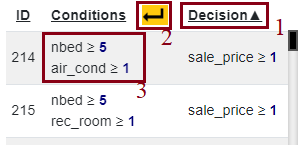
\includegraphics{figures/B-list.png}
\end{figure}

\section{Statistics}

Statistics tab is used for displaying statistics of characteristics and attributes occurring in context ruleset. When user clicks on attribute or characteristic, it will display histogram of characteristic/attributes values occurring in context ruleset.

Top attributes can be sorted by count or ``importance'' measure. ``Importance'' is a sum of attribute's occurrences in conditions multiplied by rule strength. This sum is divided by average rule strength in the data set.

\begin{figure}[H]
    \centering
    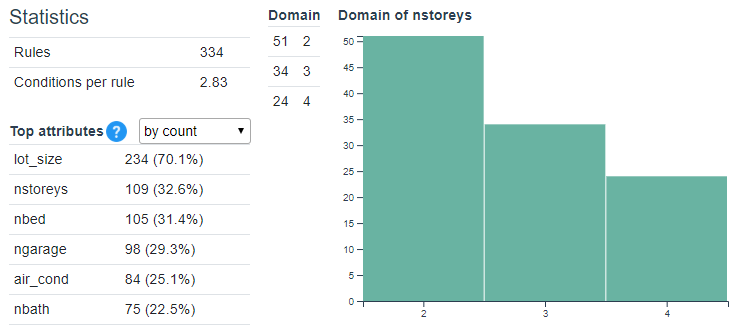
\includegraphics[width=\textwidth]{figures/B-statistics.png}
\end{figure}

\section{Attributes matrix}

Matrix of attributes is used for showing correlations between attributes. Value of matrix's element represents co-occurrence of attributes $a_i$ and $a_j$. It is the number of co-occurrences divided by: top attribute occurrences or row attribute occurrences (see Cell value option). This tab has 4 options to configure:
\begin{enumerate}
    \setlength\itemsep{0em}
    \item Contrast - every value of matrix element is raised to the power of value (contrast/10),
    \item Matrix size - enables to control visual size of matrix,
    \item Cell value - co-occurrences count is divided by top attribute's co-occurrences (Absolute) or by row attribute's occurrences (Relative to row),
    \item Cell size - Size of element is fixed (Fixed) or proportional to occurrences of attributes $a_i$ and $a_j$ (Weighted).
\end{enumerate}

\section{Rules graph}

Rules graph is used for visualizing decision rules. Nodes represent characteristics selected by user. Edges represent similarity of rules pair. There are 2 types of similarity:
\begin{itemize}
    \setlength\itemsep{0em}
    \item coverage - similarity of rules' coverage, number of objects covered by both rules divided by number of objects covered by at least one of these 2 rules, \textbf{do not confuse with rule's Coverage characteristic},
    \item semantic - similarity based on similarity of syntax of rules' conditions parts.
\end{itemize}

Semantic similarity is computed by algorithm presented below:

\begin{algorithm}[H]
    \caption{Similarity of rules pair}
    \KwIn{ruleA, ruleB}
    \myinput{attr(r) - set of attributes occuring in conditions part of rule r}
    \myinput{v(r, a) - characteristic value for condition with attribute a in rule r}
    \myinput{len(a) - length of domain of attribute a}
    \KwOut{similarity(ruleA, ruleB)}    
    % \Parameter{$\alpha \in [0,1]$}
    \BlankLine
    similarity $\gets$ 0\;
    A $\gets$ attr(ruleA)\;
    B $\gets$ attr(ruleB)\;
    
    \ForEach{$ a \in (A \cap B) $}{
        attrSimilarity $\gets 1 - \alpha \cdot \dfrac{|v(\text{ruleA}, a) - v(\text{ruleB}, a)|}{len(a)}$\;
        similarity $\gets$ similarity + attrSimilarity\;
    }
    similarity $\gets \dfrac{2 \cdot \text{similarity}}{ |A| + |B|}$ \;
\end{algorithm}

$\\ \\$
There are a lot of options for customizing rules graph:
\begin{enumerate}
    \setlength\itemsep{0em}
    \item Rules - show graph generated for rules with decision ``at least'' or with decision ``at most'',
    \item Operator - edge between nodes (rules) will exists if one of threshold (Semantic, Coverage) will be exceeded (operator = or), or if both thresholds will be exceeded (operator = and),
    \item Semantic threshold - minimum value of semantic similarity (see Operator option),
    \item Coverage threshold - minimum value of coverage similarity (see Operator option), \textbf{do not confuse with rule's Coverage characteristic},
    \item Node size - size of node is proportional to selected characteristic,
    \item Node color - color of node is proportional to selected characteristic (from white, through yellow, red, to black),
    \item Edge size - width of edge is based on selected similarity measure,
    \item Edge color - color of edge is based on selected similarity measure (from yellow through red to black),
    \item Graph mode - changes behavior when user clicks on node.
    \item Refresh - Rerun simulation (e.g. after applying filter, changing options: Thresholds, Operator, Rules, Physics),
    \item Recompute - this option should be used only for recomputing Coverage similarity after changing examples set (read more: \ref{match}).
\end{enumerate}

Physics options are options defined for forceSimulation in D3. You can also find their meaning in books about D3.
\begin{enumerate}
    \setlength\itemsep{0em}
    \item Center - strength of force that attracts nodes to the center of graph,
    \item Collide - strength of force that repels nodes from each other,
    \item Collide radius - maximum operating range of Collide force,
    \item Link - strength of force that attract nodes connected with edge,
    \item Link distance - space between nodes,
    \item Charge - strength of force that repels nodes from each other (D3 forceManyBody),
    \item Charge theta - higher theta increases speed, decreases accuracy of simulation,
    \item Iterations - Number of simulation's ticks (steps, iterations).
\end{enumerate}

\begin{figure}[H]
    \centering
    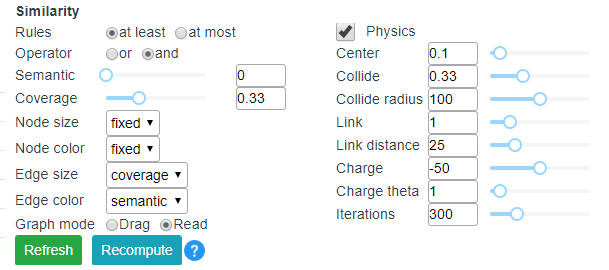
\includegraphics[width=\textwidth]{figures/B-graph.png}
\end{figure}

\end{document}
